\section{Umsetzung in Code}
Im Folgenden werde ich auf die Implementierung der einzelnen Module Schritt für Schritt eingehen und die Besonderheiten, Erfahrungen und Probleme während der Programmierung beschreiben. Ich werde argumentieren, warum ich etwas auf diese Art und Weise programmiert habe und was ich mir bei der Umsetzung gedacht habe. Um die PDF Web App auch offline nutzen zu können, habe ich die Library-Dateien runtergeladen und in einem Ordner libs direkt eingebunden, anstatt \gls{cdn}-Links zu den jeweiligen Libraries zu verknüpfen. Zur Positionierung von HTML-Elementen in der PDF Web App habe ich hauptsächlich auf das CSS Flexible Box (Flex Box) Layout zurückgegriffen. 

\subsection{Werkzeuge}
\begin{itemize}
	\item Entwicklungsumgebung: Visual Studio Code
	\item ausführende Programme: Browser Firefox, Opera, Google Chrome, Microsoft Edge
	\item Sprachen: JavaScript, CSS, HTML
	\item Libraries: Vue JS 3 Version 3.0.2, PDF-LIB, Fontkit, pdf.js, zip,js, Bootstrap Filestyle Version 2.1.0, Bootstrap Version 4.3.1, jQuery Version 3.6.0, Alwan
	\item Tutorials: Tiddly Wiki über die Bedienung der PDF Web App
\end{itemize}

\subsection{Links der Resources}
\begin{itemize}
	\item \url{https://vuejs.org/}
	\item \url{https://pdf-lib.js.org/}
	\item \url{https://www.npmjs.com/package/@pdf-lib/fontkit}
	\item \url{https://github.com/mozilla/pdf.js}
	\item \url{https://github.com/gildas-lormeau/zip.js/}
	\item \url{https://github.com/markusslima/bootstrap-filestyle}
	\item \url{https://getbootstrap.com/}
	\item \url{https://jquery.com/}
	\item \url{https://github.com/SofianChouaib/alwan}
	\item \url{https://tiddlywiki.com/}
\end{itemize}

\subsection{Ordnerstruktur}
Abbildung \ref{fig:folders} stellt die Ordnerstruktur des Projekts dar. 

\begin{figure}[!htbp]
	\centering
	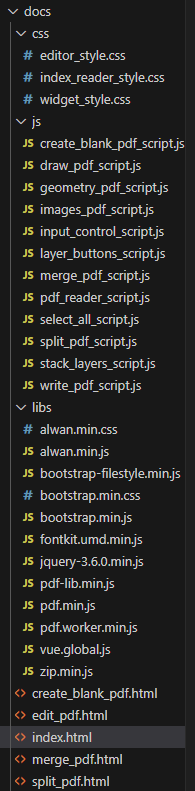
\includegraphics[width=0.3\textwidth]{"images/folders.png"}
	\caption{Ordnerstruktur der PDF Web App}
	\label{fig:folders}
\end{figure}

Im Ordner js sind meine selbst geschriebenen JavaScript-Dateien und im Ordner css meine eigenen CSS-Dateien abgelegt. Genauso wurden alle HTML-Dateien von mir erstellt. Der Ordner libs enthält alle JavaScript- und CSS-Dateien von externen Libraries. Die Datei pdf.worker.min.js ist eine dependency von pdf.js und fontkit.umd.min.js gehört zur Library PDF-LIB, um benutzerdefinierte Fonts einzubinden. Im Prinzip hat jedes Modul seine eigene JavaScript-Datei. Das Script input\_control\_script.js, welches alle Module implementiert, enthält Kontrollfunktionen für Benutzereingabefelder und die ZIP-Download-Funktionen. Der Editor enthält teilt sich die Dateien pdf\_reader\_script.js und index\_reader\_style.css mit dem Reader. Die CSS-Datei widget\_style.css deckt den Creator, Merger und Splitter ab. Der Editor besteht aus mehreren Scripten: write\_pdf\_script.js für Textelemente, draw\_pdf\_script.js für Zeichnungen, geometry\_pdf\_script.js für Shapeelemente, images\_pdf\_script.js für Bildelemente, layer\_buttons\_script.js für Ebenenmenübuttons, select\_all\_script.js für die Auswahlfilterbuttons Select All und Deselect All und stack\_layers\_script.js für Ebenenmanagementfunktionen. Der Reader, Splitter und Merger bestehen aus einer separaten HTML-Seite. Das Editormodul ist eine einzelne HTML-Seite, bei der je nach Funktion die entsprechenden Schaltflächen für die Elementoperationen mit display: flex eingeblendet und mit display: none ausgeblendet werden. 

\subsection{Layoutgestaltung}
Das Hauptmenü wollte ich sehr simpel und minimalistisch gestalten. Daher habe ich für die Startseite nur einen weißen Hintergrund mit einem oberen Balken in der Farbe \#333 als dunkles Grau, das die Hauptmenübuttons hervorhebt. Dieses dunkle Grau wird auch für die beiden oberen Reader-Leisten und den Reader Hintergrund verwendet. Die Buttons haben einen vordefinierten Style von der Library Bootstrap. In der Bootstrap Library kann man den Style durch bestimmte Klassen auswählen. Alle grünen Buttons in der PDF Web App und die Selection Menus im Creator und Splitter haben die Bootstrap-Klasse btn-success und der dunkle Button mit grüner Schrift und Umrandung des ausgewählten Hauptmenü-Buttons hat die Bootstrap Klasse btn-outline-success. Anfangs war es schwierig den default Style des input type="file" HTML-Elements zu überschreiben. Vor allem die Beschriftung des Buttons für Choose file war standardmäßig in Deutsch gehalten und lies sich nicht in englischer Sprache programmieren. Daher habe ich die Library Bootstrap Filestyle verwendet, um den Choose file Button in Englisch und mit einem Bootstrap-Style zu versehen. Um eine Designkonsistenz zu erzielen, habe ich die Bootstrap Buttons überall in der PDF Web App in verschiedenen Stylevarianten verwendet. Lediglich beim Tools Seitenmenü im Editor habe ich einen eigenen Style für die Buttons für Elementoperationen programmiert. Diese weißen Buttons haben eine schwarze Schrift mit einer Border Width von 2 Pixeln, Border Radius von 5 Pixeln und einer Border Color von \#333. Der inaktive weiße Modus-Button und die ausgeschalteten Selection Filter im Layers Menu hat den Bootstrap-Style btn-light und alle dunkelgrauen Buttons haben den Bootstrap-Style btn-dark. Alle rosa Flächen in der PDF Web App und ausgewählte Ebenen haben die Farbe \#dabdb6. Der hellgraue Operations Bar und das Namensfeld einer Ebene im Editor haben eine Farbe von \#8c8c8c. Tools und aktivierte Checkboxen haben eine türkise Hintergrundfarbe in \#5eb873. Der Hintergrund der Ebenen sowie die Seitengruppe für Layers einer Seite und das Tools Seitenmenüs hat einen Alphawert von 0.8. Abgewählte Ebenen, Selection Menus in Tools, der Hintergrund beim Output-Dateinamen und ausgewählte Dateinamen im Merger sind schwarz. Alle horizontalen Leisten mit Operationen haben eine Höhe von 58 Pixeln und dessen Buttons haben einen horizontalen Abstand von 5 Pixeln. Layers und Tools sind jeweils 190 Pixel breit. Hat man in Tools eine Font- oder Bilddatei ausgewählt, so wird nach 15 Zeichen im Dateinamen ein Zeilenumbruch eingefügt. Der Dateiname des Output-PDFs ist auf 50 Zeichen beschränkt. Im Reader befinden sich zwischen den gerenderten PDF-Seiten 20 Pixel Abstand. Alle input fields, Scrollbars und input type="checkbox" HTML-Elemente haben den default Style des Browsers. Die default Dateinamen für Reader und Editor sind wie folgt benannt: Source Dokument Dateiname, ein Unterstrich und edited. Der Creator besitzt den Dateinamen blank\_pdf und der Merger merged\_pdf. Im Splitter wird ebenfalls wie im Reader und Editor der Source Dateiname, ein Unterstrich und split verwendet. 

\subsection{Input Control}
Eine automatisierte Eingabekontrolle von Benutzereingabefeldern findet in allen Modulen, außer dem Merger, statt. Alle input fields sind input type="text" Elemente, anstatt type="number", selbst wenn nur Zahlen als Eingabewerte gültig sind. Das hat folgenden Hintergrund: Es gibt eine Funktion namens restrictInputValues, die automatisch Benutzereingaben korrigiert. Die Funktion wird ausgelöst, wenn das input field verändert wurde (change-Event). Im Prozess wird der event handler zunächst entfernt, bevor er aktiviert wird. Würde man den Event-Handler nicht zuallererst entfernen, so würde dieses Eingabefeld immer mehr Event-Handler akkumulieren. RestrictInputValues entfernt white space, wandelt die Benutzereingaben als String in Zahlen um und hält die eingegebenen Werte in einem gültigen Wertebereich. Außerdem gibt es eine Funktion convertInputToSuccess, die den Input-String in einen Zahlenwert parst und den geparsten Wert oder -1000 für eine ungültige Benutzereingabe zurückgibt. Die return value von convertInputToSuccess bestimmt maßgeblich, ob Operationen, z.B. die Schriftgröße im Texteditor ausgeführt werden sollen. Für die Eingabe von eine Liste an Seiten, gibt es eine gesonderte Funktion convertPagelistToSuccess. Hier wird im Falle von ungültigem Input die Benutzereingabe gelöscht. Eine genauere Beschreibung des Verhaltens der Input Control werde ich im Unterkapitel Testdurchführung, Abschnitt Testauswertung, weiter ausführen.

\subsection{Einlesen einer PDF-Datei}
Die Funktion für den Choose file Button ist im folgenden Codeabschnitt \ref{code:file} dargestellt:

\begin{lstlisting}[style=ES6, caption={Einlesen einer PDF-Datei}, label=code:file, breaklines=true]
	let inputFileButtons = document.getElementsByClassName('inputfile');
	for (let i = 0; i < inputFileButtons.length; i++) {
		inputFileButtons[i].addEventListener("change", function(e) {
			resetAllModes();
			// ...
			file = e.target.files[0];
			const fileReader = new FileReader(); 
			fileReader.onload = function() {
				const typedarray = new Uint8Array(this.result);
				const pdfBytes = typedarray;
				const loadingTask = pdfjsLib.getDocument(typedarray);
				loadingTask.promise.then(async (pdf) => {
					if (file.name.endsWith(".pdf")) {
						try {
							outputPDF = await PDFLib.PDFDocument.load(pdfBytes);
						} catch(encryptedErr) {
							encrypted = true;
						}
						if (!encrypted) {
							if (pdf._pdfInfo.numPages <= 5000) {
								pdfState.pdf = pdf;
								pdfState.originalPDFBytes = pdfBytes;
								pdfState.existingPDFBytes = pdfBytes;
								// ...
								pdfState.lastPage = pdf._pdfInfo.numPages;
								// ...
								adjustPDFToUserViewport();
								pdfState.renderedPage = 0;
								// ...
								let readerMode = true;
								let editorMode = false;
								const openPDFs = document.getElementsByClassName("open_pdf");
								for (let i = 0; i < openPDFs.length; i++) {
									if (openPDFs[i].classList.contains("btn-outline-success")) {
										readerMode = true;
										break;
									} else if (openPDFs[i].classList.contains("btn-success")) {
										readerMode = false;
									}
								}
								const editorBtns = document.getElementsByClassName("editor_btn");
								for (let i = 0; i < editorBtns.length; i++) {
									if (editorBtns[i].classList.contains("btn-outline-success")) {
										editorMode = true;
										break;
									} else if (editorBtns[i].classList.contains("btn-success")) {
										editorMode = false;
									}
								}
								if (!readerMode && editorMode) {
									onetimeSetup = true;
									// ...
									setTimeout(initEditor, 300);
								}
								startRender = performance.now();
								await renderPage(pageCounter, false);
							} else {
								pagesError = true;
								for (let i = 0; i < pagesErrorWidgets.length; i++) {
									pagesErrorWidgets[i].style.display = "flex";
								}
							}
						} else {
							encryptedError = true;
							for (let i = 0; i < encryptedErrorWidgets.length; i++) {
								encryptedErrorWidgets[i].style.display = "flex";
							}
						}
					}
				}).catch(unsupportedFileErr => {
					noPDFError = true;
					for (let i = 0; i < noPDFErrorWidgets.length; i++) {
						noPDFErrorWidgets[i].style.display = "flex";
					}
				});
			}
			if (file) {
				fileLoaded = true;
				fileReader.readAsArrayBuffer(file);
			}
		}, false);
	}
\end{lstlisting} 

Bei jedem Klick des Choose File Buttons werden alle Modi für aktive Operations-Buttons des Editors und andere Steuerungsmodi in der Funktion resetAllModes auf false gesetzt. Ich lese die Datei mit einem FileReader Objekt ein und führe beim load event eine Funktion aus, die am Ende das Rendern der Seiten anstößt. Die eingelesene PDF-Datei, bestehend aus einem Uint8Array, wird im Objektattribut originalPDFBytes und existingPDFBytes des globalen Objekts pdfState speichert. Die PDF-LIB-Funktionen für das Laden eines PDFs akzeptiert einen Parameter als Uint8Array und das Speichern gibt ein als Uint8Array serialisiertes PDF zurück. OriginalPDFBytes benötige ich für die Einbettung von Elementen im Editor. Im Editor wird bei jedem Downloadvorgang des modifizierten PDFs das originale PDF aus Grundlage zur Einbettung verwendet. 

Das Objekt pdfState, das den aktuellen Anzeige- und Datenstatus des eingelesenen PDFs repräsentiert, ist im Codeschnipsel \ref{code:pdfstate} dargestellt:

\begin{lstlisting}[style=ES6, caption={Objekt für den Status eines geöffnetes PDF-Dokuments}, label=code:pdfstate, breaklines=true]
	let pdfState = {
		pdf: null,
		currentPage: 1,
		lastPage: 1,
		renderedPage: 0,
		zoom: 1,
		originalPDFBytes: null,
		existingPDFBytes: null,
		originalWidths: [],
		originalHeights: []
	}
\end{lstlisting} 

Eine loadingTask wird durch die pdf.js Funktion getDocument erzeugt, die ein libraryinternes pdf Objekt zurückliefert. Dieser Return Wert wird in pdfState.pdf abgelegt und in pdfState.lastPage wird die Seitenzahl der letzten Seite gespeichert. Das pdf.js pdf-Objekt wird für das Rendern der PDF-Seiten im Reader benötigt. Weiter im Code wird das PDF dem Viewport des Browsers angepasst. Eine Anpassung erfolgt nur, wenn die Breite der ersten Seite des geöffneten Dokuments größer als der Viewport des Browsers ist. Dann wird der Zoomfaktor entsprechend angepasst, sodass die Seite mit einem Rand von 100 Pixeln formatfüllend in den Viewport passt. Anschließend wird pdfState.renderedPage initialisiert. Dieses property enthält die aktuell gerenderte Seite, die am Ende des Rendervorgangs der letzten Seite des PDFs entspricht. Ob es sich um den Reader oder Editor handelt, wird überprüft, indem ich die Bootstrap-Klassen der zugehörigen Hauptmenü-Buttons ermittle. Falls der Editor geöffnet wurde, wird er mit einer Zeitverzögerung von 300 ms aufgebaut. Hintergrund dessen ist, dass die vorherige \gls{dom}-Version erst gerendert werden muss, sonst erhält man bei Zugriff auf HTML-Collections – ein arrayähnliches Objekt – eine Länge von Null. Am Ende wird der Rendervorgang durch die rekursive, asynchrone Funktion renderPage in Gang gesetzt. Das \gls{dom} ist eine Web \gls{api} für Webdokumente wie HTML-Dokumente. Es repräsentiert die Webseite als nodes und Objekte, sodass Programmiersprachen die Dokumentenstruktur, -style und -inhalt modulieren können. Strukturell besteht das \gls{dom} aus dem \gls{dom} tree, dessen nodes den HTML-Inhalt repräsentieren. Im \gls{dom} sind alle properties, Methoden und events für die Manipulation und Erzeugung von Webseiten als Objekte organisiert \cite{mozilla-dom}. 

\subsection{Renderfunktion}
Die Funktion renderPage ist im Codeauszug \ref{code:render} abgebildet.

\begin{lstlisting}[style=ES6, caption={Renderfunktion}, label=code:render, breaklines=true]
	async function renderPage(num, renderSingle) {
		pdfState.pdf.getPage(num).then(function(page) {
			let viewport = page.getViewport({
				scale: pdfState.zoom
			});
			let viewportOriginal = page.getViewport({
				scale: 1
			});
			let canvas;
			let div;
			const pdfViewers = document.getElementsByClassName("pdf_viewer");
			for (let i = 0; i < pdfViewers.length; i++) {
				const pdfViewer = pdfViewers[i];
				// ...
				if (writeLayerStack.length < pdfState.pdf._pdfInfo.numPages) {
					div = document.createElement("div");
					div.style.display = "flex";
					div.width = viewport.width;
					div.height = viewport.height;
					div.style.width = viewport.width + "px";
					div.style.height = viewport.height + "px";
					div.style.marginBottom = "20px";
					pdfState.originalWidths.push(viewportOriginal.width);
					pdfState.originalHeights.push(viewportOriginal.height);
					div.setAttribute('data-write', pageCounter);
					div.classList.add("write_layer");
					canvas = document.createElement("canvas");
					canvas.style.display = "flex";
					canvas.width = viewport.width;
					canvas.height = viewport.height;
					canvas.style.width = viewport.width + "px";
					canvas.style.height = viewport.height + "px";
					canvas.setAttribute('data-page', pageCounter);
					canvas.classList.add("render_context");
					div.appendChild(canvas);
					pdfViewer.appendChild(div);
					writeLayerStack.push(div);
				} else if (writeLayerStack.length === pdfState.pdf._pdfInfo.numPages) {
					if (!renderSingle) {
						div = writeLayerStack[pageCounter-1];
						canvas = writeLayerStack[pageCounter-1].childNodes[0];
					} else {
						div = writeLayerStack[num-1];
						canvas = writeLayerStack[num-1].childNodes[0];
					}
					div.width = viewport.width;
					div.height = viewport.height;
					div.style.width = viewport.width + "px";
					div.style.height = viewport.height + "px";
					canvas.width = viewport.width;
					canvas.height = viewport.height;
					canvas.style.width = viewport.width + "px";
					canvas.style.height = viewport.height + "px";
				}
			}
			const context = canvas.getContext('2d');
			let renderTask = page.render({
				canvasContext: context,
				viewport: viewport
			});
			if (!renderSingle) {
				renderTask.promise.then(function() {
					pdfState.renderedPage = pageCounter;
					// ...
					pageCounter++;
					// ...
					if (pdfState.pdf != null && pageCounter <= pdfState.pdf._pdfInfo.numPages) {
						renderPage(pageCounter, false);
					}
				});
			}
		});
	}
\end{lstlisting} 

Die Funktion ruft sich rekursiv auf, falls noch nicht alle Seiten gerendert wurden. Sie kann für das Rendern auf ein oder mehreren Seiten operieren. Pro Funktionsaufruf wird der globale pageCounter hochgezählt. Mittels des pdfState.pdf-Objekts wird die aktuelle Seite geholt und ein Seitenobjekt von pdf.js entgegengenommen. Vom Seitenobjekt wird der Viewport der Seite geholt und eine Skalierung festgelegt. Das pdfState property zoom, was die aktuelle Skalierung des gesamten PDF-Dokuments speichert wird der Viewport-Skalierung zugewiesen. Viewport besitzt width und height properties. Zusätzlich wird der Viewport mit einer Skalierung von 1 geholt, damit im weiteren Verlauf von renderPage die Arrays pdfState.originalWidths und pdfState.originalHeights die Originalgröße der PDF-Seite aufnehmen können. Der Container des gerenderten PDFs besteht aus mehreren verschachtelten DIV-HTML-Elementen, wobei das innere Element die Klasse pdf\_viewer besitzt. Dem inneren PDF-Viewer-Container werden pro Ausführung von renderPage ein DIV mit der Klasse write\_layer und einem data-Attribut data-write, was die aktuelle Seitenzahl speichert, hinzugefügt. Die Write Layer symbolisiert einen Seitencontainer, der die gerenderte PDF-Seite und beigefügten Elemente des Editors enthält. Die gerenderte PDF-Seite wird in einem Canvas-Element als erstes Child der Write Layer hinzugefügt. Diese Canvas hat die Klasse render\_context und ein data-Attribut data-page für die aktuelle Seitenzahl. Sowohl die Write Layer als auch der Render Context werden in der Größe des aktuell skalierten Viewports angelegt. Die Write Layer wird zusätzlich in einem Array writeLayerStack abgelegt. WriteLayerStack hält die Write Layers in der Reihenfolge der PDF-Seiten im Dokument. Während eines erneuten Rendervorgangs wird aus diesem Array der Render Context herausgeholt und wiederverwendet. Dann wird mittels der pdf.js-Library die Seite gerendert und nach der renderTask wird eine anonyme Funktion ausgeführt. Nachdem die Seite in den Render Context geschrieben wurde, wird pdfState.renderedPage die pageCounter Variable zugewiesen. Dieses property wird dann als Maximalwert für die Input Control bei der Navigation zu einer bestimmten Seite verwendet. Folglich kann der User nur zu einer Seite springen, die ihm bereits angezeigt wird. 

\subsection{Implementierung der Vue JS 3-Module}
Die Module Creator, Splitter und Merger verwenden das Framework Vue JS 3, zwar nicht in nativer Form als \gls{spa}, jedoch wird Vue JS 3 als stand-alone widgets in diese Module integriert. Beim Creator wird annähernd die eingestellte PDF-Seitengröße als Breite und Höhe der MediaBox durch die Berechnung in den Codezeilen \ref{code:mediabox}, die ich durch Ausprobieren herausgefunden habe, gesetzt.

\begin{lstlisting}[style=ES6, caption={Berechnung der PDF-Seitengröße}, label=code:mediabox, breaklines=true]
const pageWFactor = (blankPageWidth * 1000) / 352.8;
const pageHFactor = (blankPageHeight * 1000) / 352.8;
for (let i = 0; i < blankNumOfPagesCount; i++) {
	page = pdfDoc.addPage();
	page.setMediaBox(0, 0, pageWFactor, pageHFactor);
}
\end{lstlisting} 

Beim Anklicken der Portrait-Orientierung wird in den Width and Height input fields der kleinere Wert der Seitendimensionen für die Width gesetzt und der größere Wert für die Height. Im Falle von Landscape werden Width und Height vertauscht und Quadratic orientiert sich an der Width.
\par
Wenn man den Splitter öffnet findet man zunächst einen gesperrten Save-Button vor. Der Save-Button wird erst benutzbar, wenn man eine PDF-Datei und Split-Methode im selection menu ausgewählt hat. Der Dateiname, begrenzt auf 50 Zeichen, wird unter dem Choose file-Button abgebildet. Die Methode list of pages kann man auch zum Splitten nach einer bestimmten Seite verwenden. Erst wenn man diesen Menüpunkt ausgewählt hat, wird das input field für die Seitenliste aktiviert. Die Split-Funktion fürs Splitten nach geraden und ungeraden Seiten heißt SplitAfter. Basierend auf den Rest Modulo 2 wird die Funktion nur ausgeführt, wenn bei der even pages-Split-Methode mehr als 3 Seiten im Input-PDF vorliegen bzw. bei der odd pages-Split-Methode mehr als 2 Seiten vorhanden sind. Andernfalls wird der Save-Button ebenfalls deaktiviert. Die Input-PDF Bestandteile als Dokumentobjekte von PDF-LIB, die nach jedem Split-Vorgang bei der PDF-LIB-Funktion PDFDocument.create entstehen, werden in einem globalen Array splittedPDFs gesichert. Die Arraybestandteile werden durch Klick auf Save einzeln zu einem Uint8Array serialisiert und in einem globalen Array pdfBytesList gespeichert. PdfBytesList wird dann der compressMultipleToZip funktion übergeben. Jedes gesplittete PDF enthält den Ursprungsdateinamen, einen Unterstrich und einen Index beginnend mit 0, der das Teil-PDF in der Split-Reihenfolge aufsteigend nummeriert. Alle Source-PDF-Bestandteile werden in einen ZIP-Ordner verpackt. Am Ende des Downloads werden splittedPDFs und pdfBytesList wieder als leeres Array gesetzt.
\par
Im Merger wird eine geöffnete Datei als Uint8Array einem globalen Array selectedPDFBytes hinzugefügt. Zusätzlich wird einem UL-HTML-Element, dem Dateilistencontainer, pro Datei ein LI-HTML-Element mit der Klasse file\_unselected, sowie dem Dateinamen gekürzt auf 50 Characters und einem click Event Handler für die Dateimarkierung, hinzugefügt. Erst wenn man mehr als 1 Datei oder maximal 100 ausgewählt hat werden der Save- und Remove-Button funktionstüchtig gemacht. Außerdem wird dem LI eine Reihe an drag-Events hinzugefügt: dragstart, dragover und drop. Funktion der drag-Events ist, dass der Benutzer die Listeneinträge in ihrer Reihenfolge verschieben kann. Dabei spiegelt selectedPDFBytes die Reihenfolge der Listeneinträge wieder. Für das dragging muss der Listeneintrag nicht markiert sein, jedoch beim Entfernen von einzelnen Listeneinträgen schon. Ist ein Listeneintrag schwarz markiert, so wird die Klasse file\_unselected vom entsprechenden LI entfernt und stattdessen die Klasse file\_selected hinzugefügt. Hat man so viele Listeneinträge entfernt, dass nur noch 1 oder keine Datei übrig bleibt, so wird Save abermals gesperrt. Ebenso wird Remove bei keinen Elementen deaktiviert.

\subsection{Struktur der Editorelemente}
Die 4 Editorelemente Text, Drawing, Shape und Image werden bei Erzeugung auf der Seite in 4 zugehörigen globalen Arrays in der Erstellungsreihenfolge abgelegt: userTextList für Text, drawLayerStack für Drawings, geometryPointsList für Shapes und userImageList für Images. Für die Erstellung der Editorelemente verwende ich zum einen Objekt, die die Node-Struktur der Elemente in der Webseite abbilden und zum anderen Objekte, die die elementspezifischen Eigenschaft repräsentieren. Diese Objekte werden nicht direkt verwendet, sondern sie werden als Prototypen nach dem Konzept der prototypischen Objektorientierung für die Erstellung konkreterer Objekte verwendet, die vom Prototyp erben. Im Codeabschnitt \ref{code:control-point} ist das strukturelle Prototyp-Objekt für Text, Drawing und Image abgebildet. Der darauffolgende Codeabschnitt \ref{code:shape-controller-point} zeigt das strukturelle Prototyp-Objekt für Shape.

\begin{lstlisting}[style=ES6, caption={Prototyp-Objekt für die Node-Struktur von Text, Drawing und Image}, label=code:control-point, breaklines=true]
	let controlPoint = {
		controlBox: null,
		editImg: null,
		elementToControl: null,
		type: '',
		layer: null,
		page: 1,
		x: 0,
		y: 0,
		index: 0,
		setControlPoint() {
			let div = document.createElement("div");
			div.style.position = "absolute";
			div.style.left = this.x + "px";
			div.style.top = this.y + "px";
			div.setAttribute('data-page', this.layer.getAttribute("data-write"));
			div.setAttribute('data-index', this.index);
			div.classList.add(this.type);
			div.classList.add("box");
			this.controlBox = div;
		}
	}
\end{lstlisting}

\begin{lstlisting}[style=ES6, caption={Prototyp-Objekt für die Node-Struktur von Shape}, label=code:shape-controller-point, breaklines=true]
	let shapeControllerPoint = {
		controlBox: null,
		editImg: null,
		elementToControl: null,
		layer: null,
		page: 1, 
		x: 0,
		y: 0,
		index: 0, 
		rotation: 0,
		originX: 0,
		originY: 0,
		setControlPoint() {
			let div = document.createElement("div");
			div.style.position = "absolute";
			div.style.left = this.x + "px";
			div.style.top = this.y + "px";
			div.setAttribute('data-page', this.layer.getAttribute("data-write"));
			div.setAttribute('data-index', this.index);
			div.classList.add("shape");
			div.classList.add("box");
			this.controlBox = div;
		},
		rotateControlPoint() {
			this.controlBox.style.marginLeft = this.originX + "px";
			this.controlBox.style.marginTop = this.originY + "px";
			this.controlBox.style.transform = "rotate(" + this.rotation + "deg)";
		}
	}
\end{lstlisting}  

Vom controlPoint-Prototyp leitet das Objekt controlP ab und von shapeControllerPoint leitet shapeControllerP ab. ShapeControllerPoint stellt einen spezialisierten controlPoint dar, der mit Rotationseigenschaften erweitert wurde. ControlP und shapeControllerP-Objekte werden direkt in userTextList, drawLayerStack, userImageList und geometryPointsList gespeichert.
Die Prototypen besitzen ein Attribut elementToControl, um die Objekte mit elementspezifischen Eigenschaften zu speichern. Dessen Prototypen heißen userText für Text, drawLayer für Drawings, shape für Shapes und userImage für Images. Sie sind in den Codesegmenten aufgeführt.

\begin{lstlisting}[style=ES6, caption={Prototyp-Objekt für die textspezifischen Eigenschaften}, label=code:user-text, breaklines=true]
	let userText = {
		pdfDoc: null,
		pdfBytes: null,
		text: '',
		x: 1,
		y: 1,
		size: 1,
		fontKey: null,
		font: null,
		lineHeight: 34,
		color: rgb(0, 0, 0),
		page: 1,
		opacity: 1.0,
		rotation: degrees(0),
		setTextElem() {
			this.pdfDoc.getPages()[0].drawText(this.text, {
				x: this.x,
				y: this.y,
				size: this.size,
				font: this.font,
				color: this.color,
				lineHeight: this.lineHeight,
				rotate: this.rotation
			});
		}
	}
\end{lstlisting}

\begin{lstlisting}[style=ES6, caption={Prototyp-Objekt für die drawingspezifischen Eigenschaften}, label=code:draw-layer, breaklines=true]
	let drawLayer = {
		paths: [],
		currentPathIndex: 0, 
		rotation: 0,
		wasRotated: false
	}
\end{lstlisting}

\begin{lstlisting}[style=ES6, caption={Prototyp-Objekt für die shapespezifischen Eigenschaften}, label=code:shape, breaklines=true]
	let shape = {
		context: null,
		type: "",
		x: 0,
		y: 0,
		xp2: 50,
		yp2: 50,
		width: 100,
		height: 100,
		stroke: 'rgba(0,0,0,1.0)',
		strokeWidth: 3,
		fill: '',
		useFill: false,
		useStroke: false,
		rotation: 0,
		page: 1,
		drawShape() {
			if(this.type === "rectangle") {
				let rectCenterX = this.x + this.width / 2;
				let rectCenterY = this.y + this.height / 2;
				this.context.save();
				this.context.beginPath();
				this.context.translate(rectCenterX, rectCenterY);
				this.context.rotate(this.rotation * Math.PI / 180);
				this.context.translate(-rectCenterX, -rectCenterY);
				if (this.useFill) 
				this.context.fillStyle = this.fill;
				if (this.useStroke) {
					this.context.strokeStyle = this.stroke;
					this.context.lineWidth   = this.strokeWidth;
				}
				if (this.useFill) {
					this.context.fillRect(this.x, this.y, this.width, this.height);
				}
				if (this.useStroke) {
					this.context.strokeRect(this.x, this.y, this.width, this.height);
				}
				this.context.restore();
			} else if (this.type === "triangle") {
				let triCenterX = this.x + this.width / 2;
				let triCenterY = this.y + this.height / 2;
				this.context.save();
				this.context.beginPath();
				this.context.translate(triCenterX, triCenterY);
				this.context.rotate(this.rotation * Math.PI / 180);
				this.context.translate(-triCenterX, -triCenterY);
				this.context.moveTo(this.x, this.y);
				this.context.lineTo(this.x, this.y + this.height);
				this.context.lineTo(this.x + this.xp2 + this.width, this.y + this.yp2);
				this.context.closePath();
				
				if (this.useFill) 
				this.context.fillStyle = this.fill;
				
				if (this.useStroke) {
					this.context.strokeStyle = this.stroke;
					this.context.lineWidth   = this.strokeWidth;
				}
				
				if (this.useFill) 
				this.context.fill();
				
				if (this.useStroke)    
				this.context.stroke();
				
				this.context.restore();
			} else if (this.type === "circle") {
				this.context.beginPath();
				this.context.ellipse(this.x, this.y, this.width / 2, this.height / 2, this.rotation * Math.PI / 180, 0, 2 * Math.PI);
				
				if (this.useFill) {
					this.context.fillStyle = this.fill;
				}
				if (this.useStroke) {
					this.context.strokeStyle = this.stroke;
					this.context.lineWidth   = this.strokeWidth;
				}   
				this.context.closePath();
				if (this.useFill) {
					this.context.fill();
				}
				if (this.useStroke)    
				this.context.stroke();
			}
		}
	}
\end{lstlisting}

\begin{lstlisting}[style=ES6, caption={Prototyp-Objekt für die imagespezifischen Eigenschaften}, label=code:user-image, breaklines=true]
	let userImage = {
		pdfDoc: null,
		pdfBytes: null,
		image: null,
		base64String: "",
		type: "",
		x: 1,
		y: 1,
		width: 1,
		height: 1,
		page: 1,
		opacity: 1.0,
		rotation: degrees(0),
		setImageElem() {
			this.pdfDoc.getPages()[0].drawImage(this.image, {
				x: this.x,
				y: this.y,
				width: this.width,
				height: this.height,
				rotate: this.rotation,
			});
		}
	}
\end{lstlisting}

Die spezifischen Objekte zu ihren Prototypen heißen currentUserText für userText, drawingLayer für drawLayer, currentShape für shape und currentUserImage für userImage. Sowohl die Nodestrukturobjekte, als auch die Eigenschaftsobjekte werden beim Hinzufügen von Elementen erstellt und mit Standardwerten initialisiert. 

\subsection{Aufbau eines PDF-Seitencontainers}
Die Wurzel eines PDF-Seitencontainer bildet ein DIV mit der Klasse write\_layer. Die write\_layer hat mindestens ein child, eine Canvas mit der Klasse render\_context. Dieser Fall liegt vor, wenn man noch keine Elemente zum PDF hinzugefügt hat. Man kann sich den Render Context als Zeichenfläche vorstellen, die durch die Dimensionen der PDF-Seite begrenzt ist, mit dem gerenderten Seiteninhalt als Hintergrund. Sobald der Benutzer Elemente der Seite hinzufügt, werden weitere Schichten auf den Render Context gelegt, wobei ein Element aus einer Canvas, die ich editimg genannt habe, für die Darstellung und einem 40 x 40 Pixel-großen DIV namens controlBox für den Kontrollpunkt des Elements besteht. Die Canvas besitzt 3 Klassen: Editimg, visible und eine Elementtyp-Klasse. Die Klasse editimg bezeichnet die Canvas, die das gerenderte, einzelne Element enthält. Visible definiert den Sichtbarkeitsstatus für das Ein- und Ausblenden von Elementen über die Ebenensteuerung. Die Typklasse kann entweder text, drawing, shape oder image sein. Jedes editimg enthält außerdem ein data-page für die Seitenzahl und data-index für die Position in der Elementliste Attribut. Die Größe des editimgs entspricht immer der Größe des zugehörigen render\_contextes. Auf der controlBox habe ich eine Reihe von Event-Handler definiert, die die Operationen im Operations Bar und Tools ausführen. Sie besitzt eine Typklasse und die Klasse box, um alle controlBoxes im Dokument ansprechen zu können. Die controlBox besitzt ebenfalls die gleichen data-Attribute wie das zugehörige editimg. Die editimgs werden bei Erzeugung aufeinander gestapelt mit dem zuletzt erstellten editimg zuoberst. Alle editimgs werden in einem Gruppierungs-DIV mit der Klasse editimg\_group akkumuliert. Ebenfalls werden alle controlBoxes in einem gruppierenden DIV mit der Klasse control\_group vereint. Die editimg\_group liegt über dem render\_context. Ganz oben befindet sich die control\_group, damit Kontrollpunkte nicht von gerenderten Elementen verdeckt werden. Die control\_group und editimg\_group werden beim Hinzufügen des ersten Elementes auf der Seite erstellt. Jede write\_layer hat jeweils eine editimg\_group und control\_group. Das Node-Tree Segment für den Aufbau einer write\_layer ist in Screenshot \ref{fig:write-layer} veranschaulicht. 

\begin{figure}[!htbp]
	\centering
	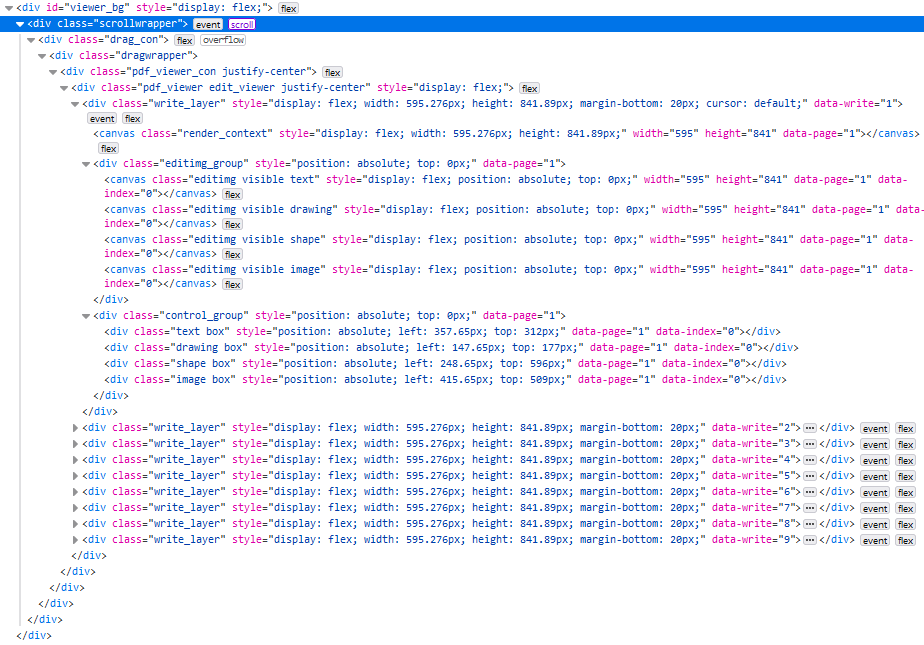
\includegraphics[width=1\textwidth]{"images/write-layer.png"}
	\caption{Node-Tree Segment für den Aufbau einer write\_layer mit 4 Elementen jedes Typs}
	\label{fig:write-layer}
\end{figure}

Für editimg und controlBox gibt es properties in den Nodestrukturobjekten. Dort wird die Canvas und das DIV abgespeichert. Außerdem gibt es ein layer property, in dem die zugehörige write\_layer gesichert wird. In den properties type wird der Elementtyp als String hinterlegt, page beschreibt die Seitenzahl, x und y sind die Koordinaten auf der Seite und index ist die Position des Elements in der zugehörigen Liste. Die Reihenfolge der Elemente in userTextList, drawLayerStack, geometryPointsList und userImageList ändert sich nie, es sei denn ein Element wird vom Benutzer gelöscht. Der index in den Nodestrukturobjekten muss immer mit data-index von editimg und controlBox übereinstimmen. Über diesen maßgeblichen index kann auf das Element in der jeweiligen Liste zugegriffen werden.

\subsection{Hinzufügen von Elementen}
Jedes Element hat seine separate Funktion, um es der Seite hinzuzufügen. Jede Funktion enthält die Funktion createStackLayer, um eine Layer für das Element zu erstellen. Am Ende jeder Funktion zum Hinzufügen wird das Nodestrukturobjekt der zugehörigen Liste hinzugefügt. Wenn Text hinzugefügt werden soll, wird der Text in Form des Eigenschaftsobjekt erstellt. Aus Sicht der Implementierung wird ein PDF-Dokument mit einer Seite mit PDF-LIB erstellt, worauf der Text an der Stelle, wo der Benutzer mit der Maus auf die Seite geklickt hat, platziert wird. Die einzelne PDF-Seite hat die Größe des render\_contextes bzw. der write\_layer, da der render\_context und die write\_layer die gleiche width und height haben. Dann wird diese Seite mit einem transparenten Hintergrund mit pdf.js in das editimg gerendert. Das Klick-Event ist mit der write\_layer verknüpft. Alle Funktionen zum Hinzufügen von Elementen sind an das Klick-Event auf der write\_layer gebunden. In die PDF-Seite wird der Standard-Font TimesRoman eingebettet. Im Eigenschaftsstrukturobjekt befindet sich die PDF-LIB-Funktion drawText und sie wird in addText mit Standardwerten gefüttert. Zu beachten ist, dass currentUserText.opacity nicht an drawText übergeben wird, da die opacity-Implementierung der PDF-LIB in der Library defekt zu sein scheint. Außerdem wird das Dokument-Objekt von PDF-LIB in currentUserText.pdfDoc abgelegt und die Uint8Array-Repräsentation des Dokuments ebenfalls. Die Seitenzahl wird in currentUserText.page abgelegt und die currentUserText.rotation mit 0 initialisiert. Alle Editor-Elemente werde bei der Erzeugung mit einer Rotation von 0 erstellt und alle Eigenschaftsobjekte haben ein page property. Des Weiteren wird der Textinhalt als String in currentUserText.text festgehalten, das Font-Objekt, das beim Einbetten des Fonts entsteht, in currentUserText.font, sowie die ArrayBuffer-Variante des, mit dem Dateibrowser geöffneten Fonts, in currentUserText.fontKey gespeichert. Text-Eigenschaftsobjekte sind die einzigen Eigenschaftsobjekte mit einem size Attribut.
\par
Die Funktion addImage funktioniert ähnlich wie addText. Das Image wird ebenfalls auf eine PDF-Seite platziert und mit transparentem Hintergrund in editimg gerendert. Im Vorgang wird das eingelesene Image, was in der Bilddateiliste in Tools ausgewählt wurde, in Form von Base64 in das einseitige PDF eingebettet. Zurückgegeben wird ein Bildobjekt von PDF-LIB, was in currentUserImage.image abgelegt wird. Das erzeugte PDF-Objekt wird in currentUserImage.pdfDoc und das Base64-Image in currentUserImage.base64String gespeichert. Shape- und Image-Eigenschaftsobjekte haben width und height Attribute. In currentUserImage befindet sich die setImageElem-Methode mit der drawImage-PDF-LIB-Funktion.
\par
Shapes und Drawings benötigen keine PDF-Dokumentseite bei ihrer Entstehung. Der shapeControllerP besitzt noch properties rotation, originX, originY und eine Funktion rotateControlPoint, um die controlBox mit dem Shape gemeinsam im gleichen Winkel zu drehen. In der Funktion addingShape wird der Shape direkt auf das editimg mit Canvas-Funktionen für Rechtecke und Ellipsen gezeichnet. Dreiecke müssen durch einzelne Linien gezeichnet werden. In currentShape.context wird der Canvas 2D-Rendering-Context gespeichert. Er wird für die Zeichenoperationen verwendet. CurrentShape.type speichert den Shape-Typ als String. Die Typen heißen rectangle, triangle und circle. Die properties xp2 und yp2 stehen für den dritten Punkt des Dreiecks (Triangle's 3rd Point). Sie werden nur bei Erstellung von Triangles initialisiert und bei der Triangle's 3rd Point Operation verwendet. CurrentShape besitzt stroke, strokeWidth, fill, useFill und useStroke Attribute. UseFill und useStroke werden für die Steuerung der Checkboxen in der GUI bei Stroke Color und Fill Color in Tools verwendet. Man kann entweder nur eine Stroke Color oder nur eine Fill Color anwenden oder beide gleichzeitig. 
\par 
Die Funktion zum Hinzufügen von Drawings heißt draw und ist mit dem Klick-Event auf die write\_layers verbunden. Im drawLayer.paths-Array werden die Pfadpunkte des Zeichenvorgangs angehängt. Zuerst wird geprüft, ob sich auf der Seite schon ein Drawing befindet, falls nicht wird ein controlP und eine drawingLayer erstellt. Sie wird ebenfalls erstellt, wenn der Benutzer New Layer gedrückt hat. Gezeichnet wird auf der selektierten Layer. Wenn keine DrawingLayer selektiert ist wird standardmäßig auf der zuletzt gezeichneten Layer der Seite gemalt. Bei der Erstellung der Pfadsegmente wird, wie bei Shape, direkt auf dem context des editimgs gezeichnet und in drawingLayer.paths wird ein Objekt mit den x, y, line, color und compositeOp properties hinzugefügt. DrawingLayer.currentPathIndex dient der Traversierung von paths. Gezeichnet wird mit einem context.lineCap "round" und context.lineJoin "round" Linienaussehen, d.h. die Linie ist abgerundet an ihren Enden. Die context.globalCompositeOperation ist "source-over". Beim Radieren wäre sie "destination-out". Diese globalCompositeOperation wird in compositeOp in paths vermerkt. Die erase-Funktion funktioniert ähnlich wie draw, nur dass keine Layers, controlPs und DrawingLayers erstellt werden. Diese Objekte werden nur in draw erstellt.


\subsection{Erzeugung von Layers}
















\subsection{Implementierung des Zooms}

\subsection{Downloadfunktion}















